\documentclass[a4paper,11pt,openright,twoside]{report}

\usepackage{graphics}
\usepackage[british,UKenglish,USenglish,american]{babel}
\usepackage[infoshow,debugshow]{tabularx}
\usepackage{url,amsfonts,epsfig}
\usepackage{tabularx}
\usepackage{amsmath}
\usepackage{newlfont}
\usepackage{booktabs}
\usepackage{caption} 
\usepackage{titlesec}
\usepackage{braket}
\usepackage{subfig}
\usepackage{ragged2e}
\captionsetup{tableposition=top,figureposition=bottom,font=small}
\usepackage[a4paper,bottom=2cm,top=2cm,headheight=14pt,includehead,includefoot,marginparwidth=4cm,marginparsep=0.5cm,inner=2cm,outer=5cm,heightrounded]{geometry}

\setlength{\voffset}{-0.5in}
\setlength{\topmargin}{-0.2in}
\setlength{\textheight}{240mm}
\setlength{\textwidth}{142mm}
\setlength{\evensidemargin}{0.3in}
\setlength{\oddsidemargin}{0.3in}
\setlength{\parindent}{0pt}

\begin{document}
\begin{minipage}[b]{0.20\textwidth}    %% b or t, default is c
	\centering
	
\includegraphics[height=2.5cm]{images/unipd}
\end{minipage}%
\begin{minipage}[b][2cm]{0.6\textwidth}
	\centering\large \sc
	University of Padua \vfill
	Degree Course in \\ ICT for Internet and Multimedia\vfill
	\small Academic Year 2017/2018 \end{minipage}%
\begin{minipage}[b]{0.20\textwidth}
	\centering 
	
\includegraphics[height=2.5cm]{images/dei}
\end{minipage}

\vspace*{20pt}
\begin{center}\leavevmode
	\normalfont
	{\huge\raggedleft \bfseries\textsf{ \boldmath{$1^{st}$} Homework}\par}%
	\hrulefill\par
	{\LARGE\raggedright \textsf{\bfseries SANTI GIOVANNI - 1177739}\par}%
	%    {\Large \@date\par}%
	\vspace*{20pt}
	{\LARGE\raggedright \textsf{\bfseries VANIN EDOARDO - 1179018}\par}%
	%    {\Large \@date\par}%
	\vspace*{20pt}
\end{center}	
	
\section*{PROBLEM 1}
Given a single realization of 800 i.i.d. samples of the r.p $ \left\lbrace x(k) \right\rbrace$ defined by:
\begin{equation*}
x(k) = e^{j(2 \pi f_1k+\varphi_1)}+0.8e^{j(2 \pi f_2k+\varphi_2)}+w(k)
\end{equation*}
where $w(k)\sim \mathcal{CN}(0,\sigma_w^2)$, $f_1=0.17$, $f_2 = 0.78$, $\sigma_w^2=2.0$ $\varphi_{1,2}\sim \mathcal{U}(0,2\pi)$ are statistically independent, we want to estimate the $\mathcal{PSD}$ of $ \left\lbrace x(k) \right\rbrace$ using the following models:

\subsection*{BLACKMAN AND TUKEY CORRELOGRAM}
\begin{equation}
\mathcal{P}(F) = T_c \sum_{n=-L}^{L} w(n)\hat{r}_x(n)e^{-j2\pi fnT_c}
\end{equation}
where $\hat{r}_x(n)$ is the autocorrelation of x taken from -L to L and $w(n)$ is a Hamming window of length 2L+1. The autocorrelation function is evaluated using the \textit{unbiased estimate} give by:
\begin{equation*}
\hat{r}_x(n) = \frac{1}{K-n}\sum_{k=n}^{K-1}x(k)x^*(k-n) \quad \quad n = 0,1,...,K-1
\end{equation*}
where K is the number of samples. In ordert to reduce the variance of the estimate, we chose $L=\lfloor \frac{K}{5} \rfloor$. The hamming window is defined by:
\begin{equation}\label{ham}
w(k) = \begin{cases}
       0.54 + 0.46 \cos \left(2\pi \frac{k-\frac{D-1}{2}}{D-1} \right) \quad \quad k=0,1,...,D-1 \\
       0 \quad \quad \quad \quad \quad \quad \quad \quad \quad\quad \quad \quad \quad \quad elsewhere
       \end{cases}
\end{equation} 


\subsection*{PERIODOGRAM}
\begin{equation}\label{Per}
\mathcal{P}_{PER}(f) = \frac{1}{KT_c} | \tilde{\mathcal{X}}(f) |
\end{equation}
where $\tilde{\mathcal{X}}(f) = T_c \mathcal{X}(f)$, $\mathcal{X}(f)$ is the Fourier Transform of $ \left\lbrace x(k) \right\rbrace$, $k = 0,1,...,K-1$.

\subsection*{WELCH PERIODOGRAM}
\begin{equation}
\mathcal{P}_{WE}(F) = \frac{1}{N_s}\sum_{x=0}^{N_s-1}\mathcal{P}_{PER}^{(s)}(f)
\end{equation}
where $\mathcal{P}_{PER}^{(s)}(f)$ is the periodogram estimate given by Eq.\ref{Per}.  
The model extracts different subsequences of consecutive D samples which eventually overlap. If $x^{(s)}$ is the s-th subsequence, characterized by S samples in common with the previous subsequence $x^{(s-1)}$ and with the following $x^{(s+1)}$, the total number of subsequences is $N_s = \lfloor \frac{K-D}{D-S}-1 \rfloor$. In our analysis, we chose S=?? and D=??. \\
More in details, we computed:
\begin{equation*}
\begin{split}
x^{(s)}(k) &= w(k)x(k+s(D_S))   \quad \quad k=0,1,...,D-1 \quad s = 0,1,...,N_s-1 \\
\tilde{\mathcal{X}}^{(s)}(f) &= \mathcal{F}[x^{(s)}(k)] = T_c\sum_{k=0}^{D-1}x^{(s)}(k)e^{-j2 \pi fkT_c} \\
\mathcal{P}^{(s)}_{PER}(f) &= \frac{1}{DT_cM_w} \left | \tilde{\mathcal{X}}^{(s)}(f) \right |^2
\end{split}
\end{equation*}
where $w(k)$ is the hamming window difined by Eq. \ref{ham} and $M_w = \frac{1}{D}\sum_{k=0}^{D-1}w^2(k)$ is the normalized energy of the window.

\subsection*{AR(N) MODEL}
%\begin{figure}
%	\centering
%	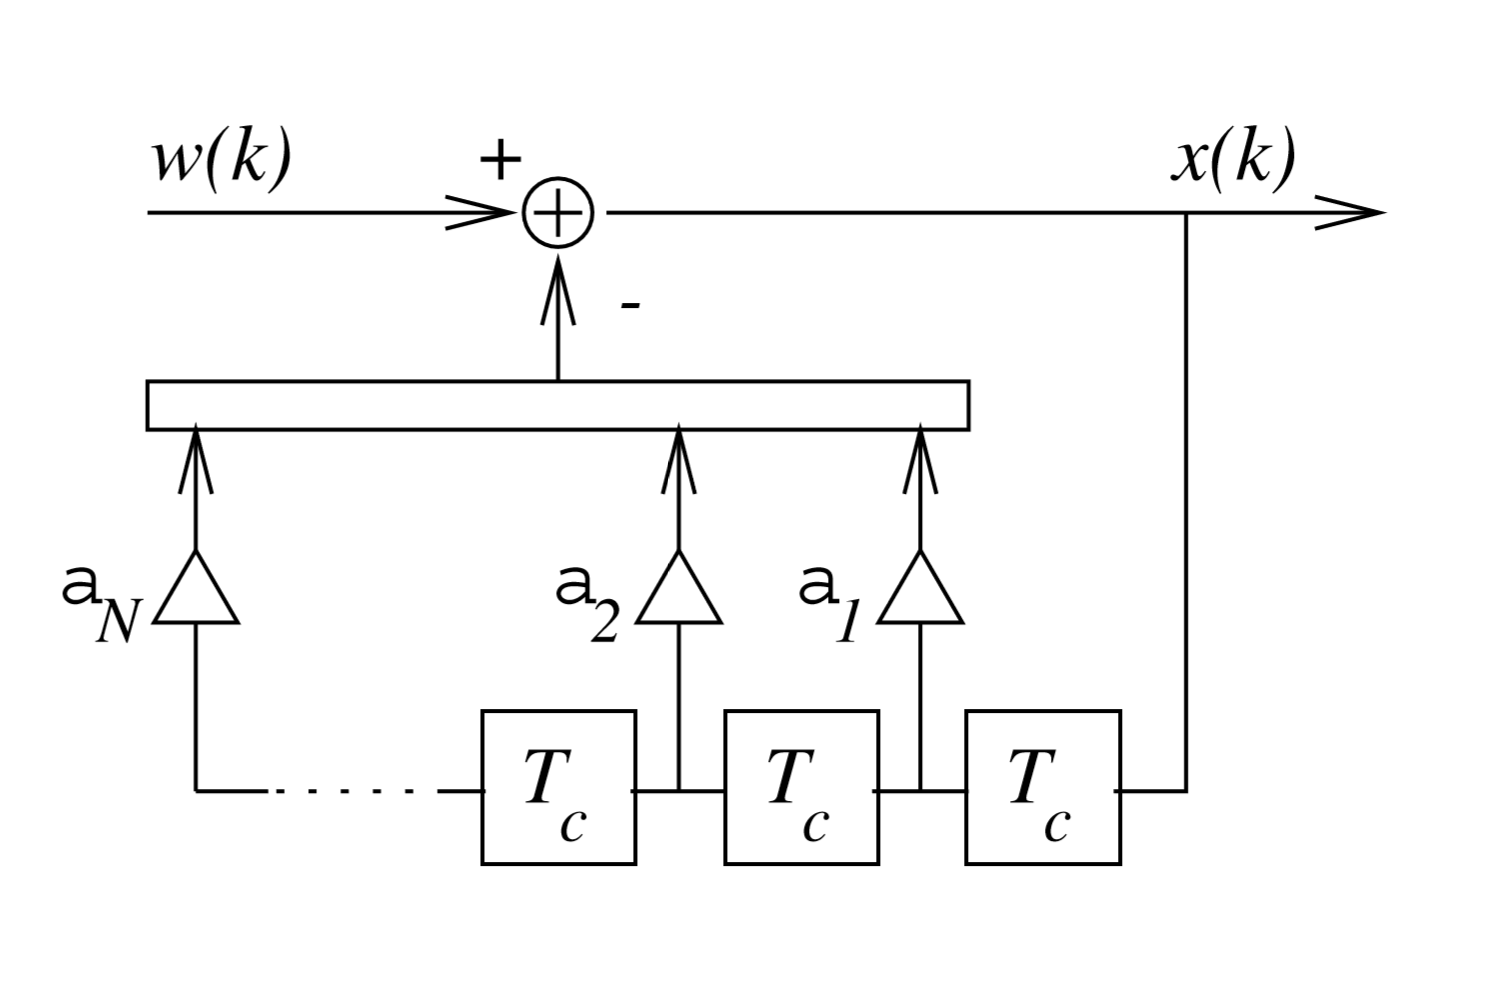
\includegraphics[width=5cm]{AR}
%	\caption{AR model of a process x.}\label{AR} 
%\end{figure}
\begin{equation}\label{E_AR}
\mathcal{P}_{AR}(f) = \frac{T_c \sigma_w^2}{\left | \mathcal{A}(f) \right |^2}
\end{equation}
The output process is described by the following recursive e equation
\begin{equation}\label{coeff}
x(k) = -\sum_{n=1}^{N} a_nx(k-n)+w(k)
\end{equation}
where $w$ is white noise with variance $\sigma_w^2$. The transfer function of this system is given by
$ H_{AR} = \frac{1}{A(z)} $ where $ A(z) = 1+\sum_{n=1}^Na_nz^{-n}$. The ACS of \textit{x} in z-domain is easily evaluated using 
\begin{equation*}
P_x(z) = \frac{\sigma_w^2}{A(z)A^*(\frac{1}{z^*})}
\end{equation*}
from which Eq. \ref{E_AR} is computed letting $\mathcal{A}(f) = A(e^{j2\pi f T_c})$. \\
Coefficients $a_1,a_2,...,a_N$ are computed exploiting the \textit{Yule-Walker equation}
 $\mathbf{a} = -\mathbf{R}^{-1}\mathbf{r}$, where $ r = \left[ r(1),r(2), \dots, r(N) \right] $ and the \textit{autocorrelation matrix} is defined as
\begin{equation*}
\mathbf{R} = \begin{pmatrix}
    r(0) & r(-1) & \dots & r(_N+1) \\
    r(1) & r(0) & \dots & r(-N+2) \\
    \vdots & \vdots & \ddots & \vdots \\
    r(N-1) & r(N-2) &  \dots & r(0)
    \end{pmatrix}
\end{equation*}
The noise variance deriving from the model is 
\begin{equation}\label{sigmaw}
\sigma_w^2 = r_x(0) + \mathbf{r}^H\mathbf{a}
\end{equation}

\subsection*{CONCLUSIONS}
A comparison between different PSD estimates of $ \left\lbrace x(k) \right\rbrace$ is now discussed. The difficulties in this problem were related to the fact that the noise variance is double with respect to the maximum amplitude of the usefull signal. For this reason, a good analysis can be achieved only by considering a generated sequence $ \left\lbrace x(k) \right\rbrace$ which is not too corrupted at the carriers frequencies $f_1$ and $f_2$. The four different PSD estimates are shown in Figure [\ref{PSD}]. \\

\begin{figure}
	\centering
	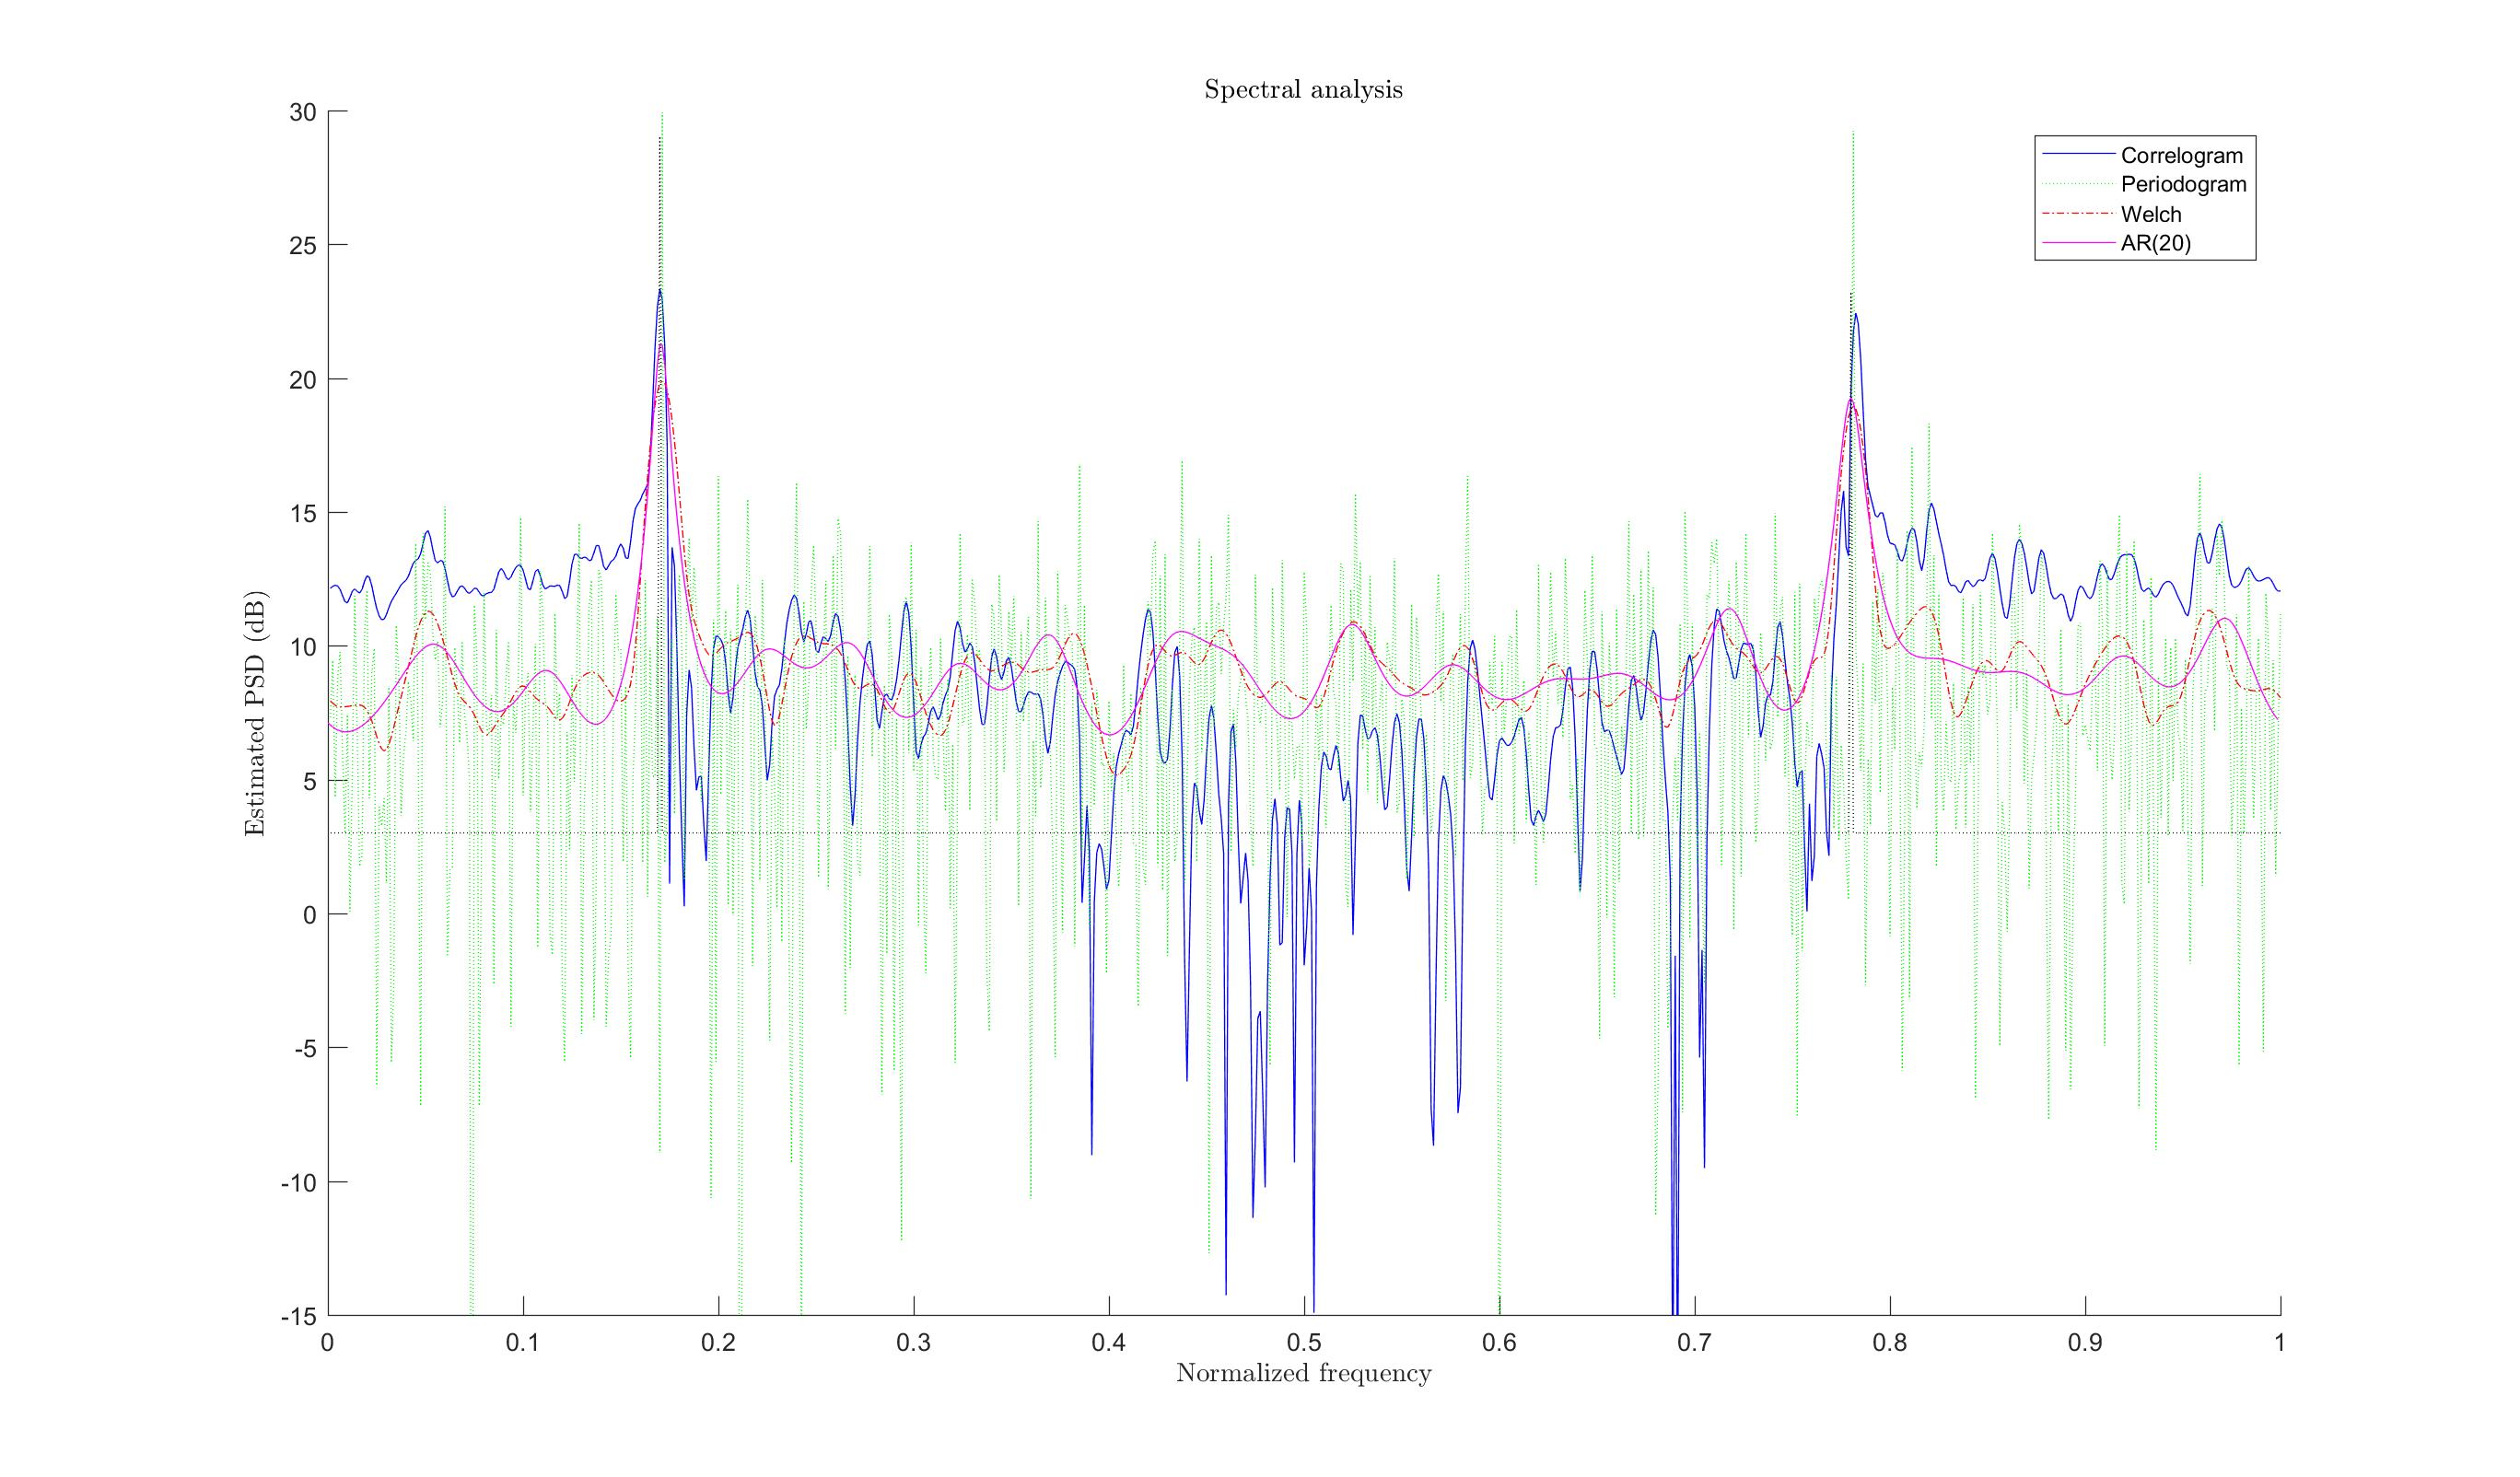
\includegraphics[width=14cm]{images/PSD.jpg}
	\caption{PSD estimates.}\label{PSD} 
\end{figure}

The parameters of the different models are as follow. The order of the autocorrelation estimator for the Correlogram is $ N_{corr} = \lfloor K/5 \rfloor = 160 $, and the window used is a Hamming window definde in Eq. \ref{ham}. For the Periodogram the window used is the rectangular one, while for the Welch Periodogram we set $D=??$ and $S=??$ still using an Hamming window. This choise was made by observing different PSD estimates with varying values of S and D, as shown in Figure [\ref{WelchSD}]. The order evaluation for the AR model was carried out by analysing the behaviour of the noise variance $\sigma_w^2$ with varying N defined in eq. \ref{sigmaw} and graphically shown in Fig. [\ref{sigmavsN}].

\begin{figure}
	\centering
	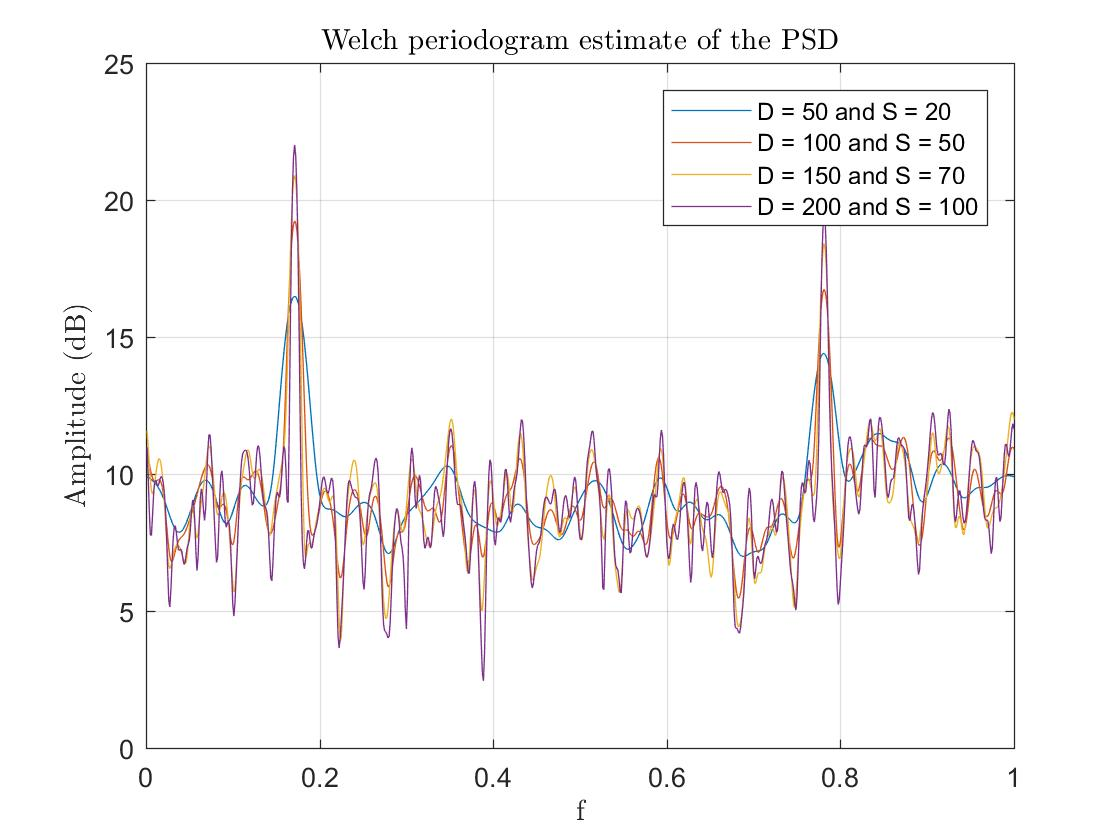
\includegraphics[width=14cm]{images/Welch_vs_SD.jpg}
	\caption{Welch periodogram estimates as a function of different values of D and S.}\label{WelchSD}
\end{figure}
\begin{figure}[h]
	\centering
	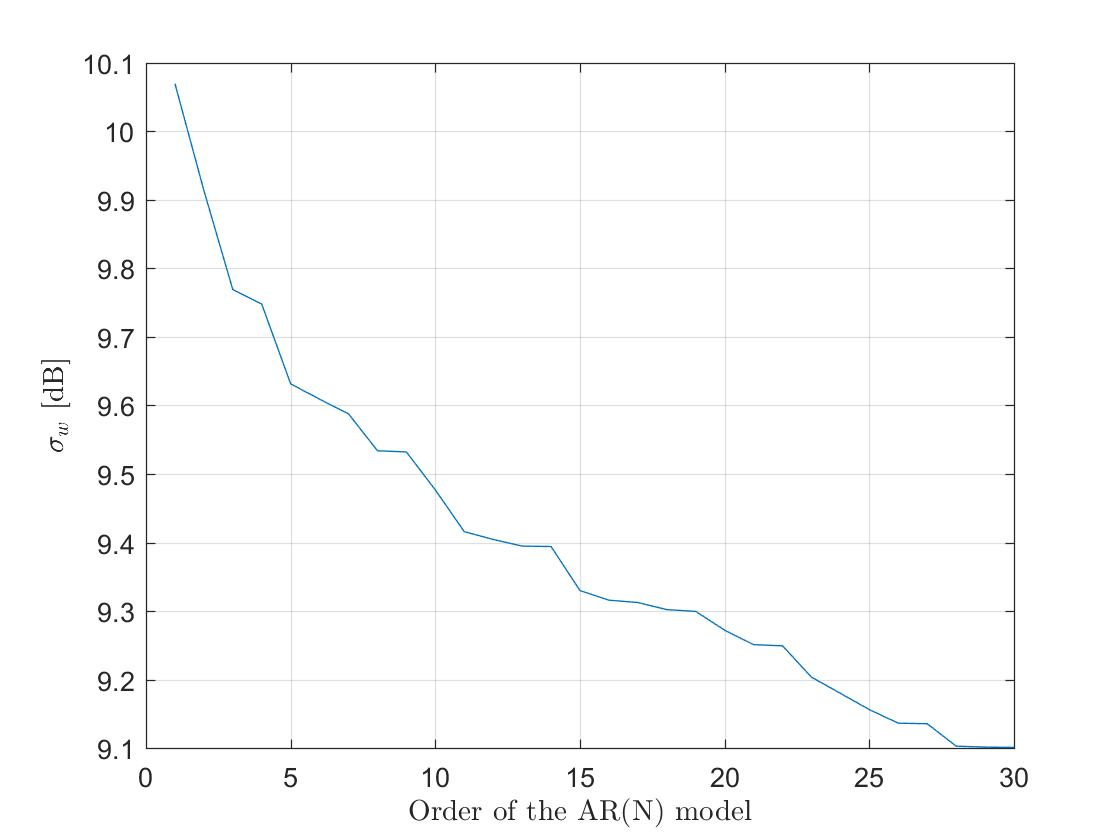
\includegraphics[width=14cm]{images/sigma_vs_N.jpg}
	\caption{Variance of the AR model white noise as a function of the order N.}\label{sigmavsN}
\end{figure}

It is easy to see that no significant keen occurs neither for high value of N, thus for this problem there is not a clean value that should be chosen. On the other hand, a large N may result in an ill-conditioned autocorrelation matrix $\mathbf{R}$, this because of the presence of spectral lines in the original process.
For all these reasons, we decided that N=?? was a good trade-off.

\clearpage
\section*{PROBLEM 2}
The only differen with Problem 1 is the noise variance, which is $\sigma_w=0.1$. However, now the noise component is almost negligible with respect the usful signal, and then we were able to provide a much more accurate analysis. The different spectral estimates are given in Figure [\ref{PSD_2}]. \\

\begin{figure}[h!]
	\centering
	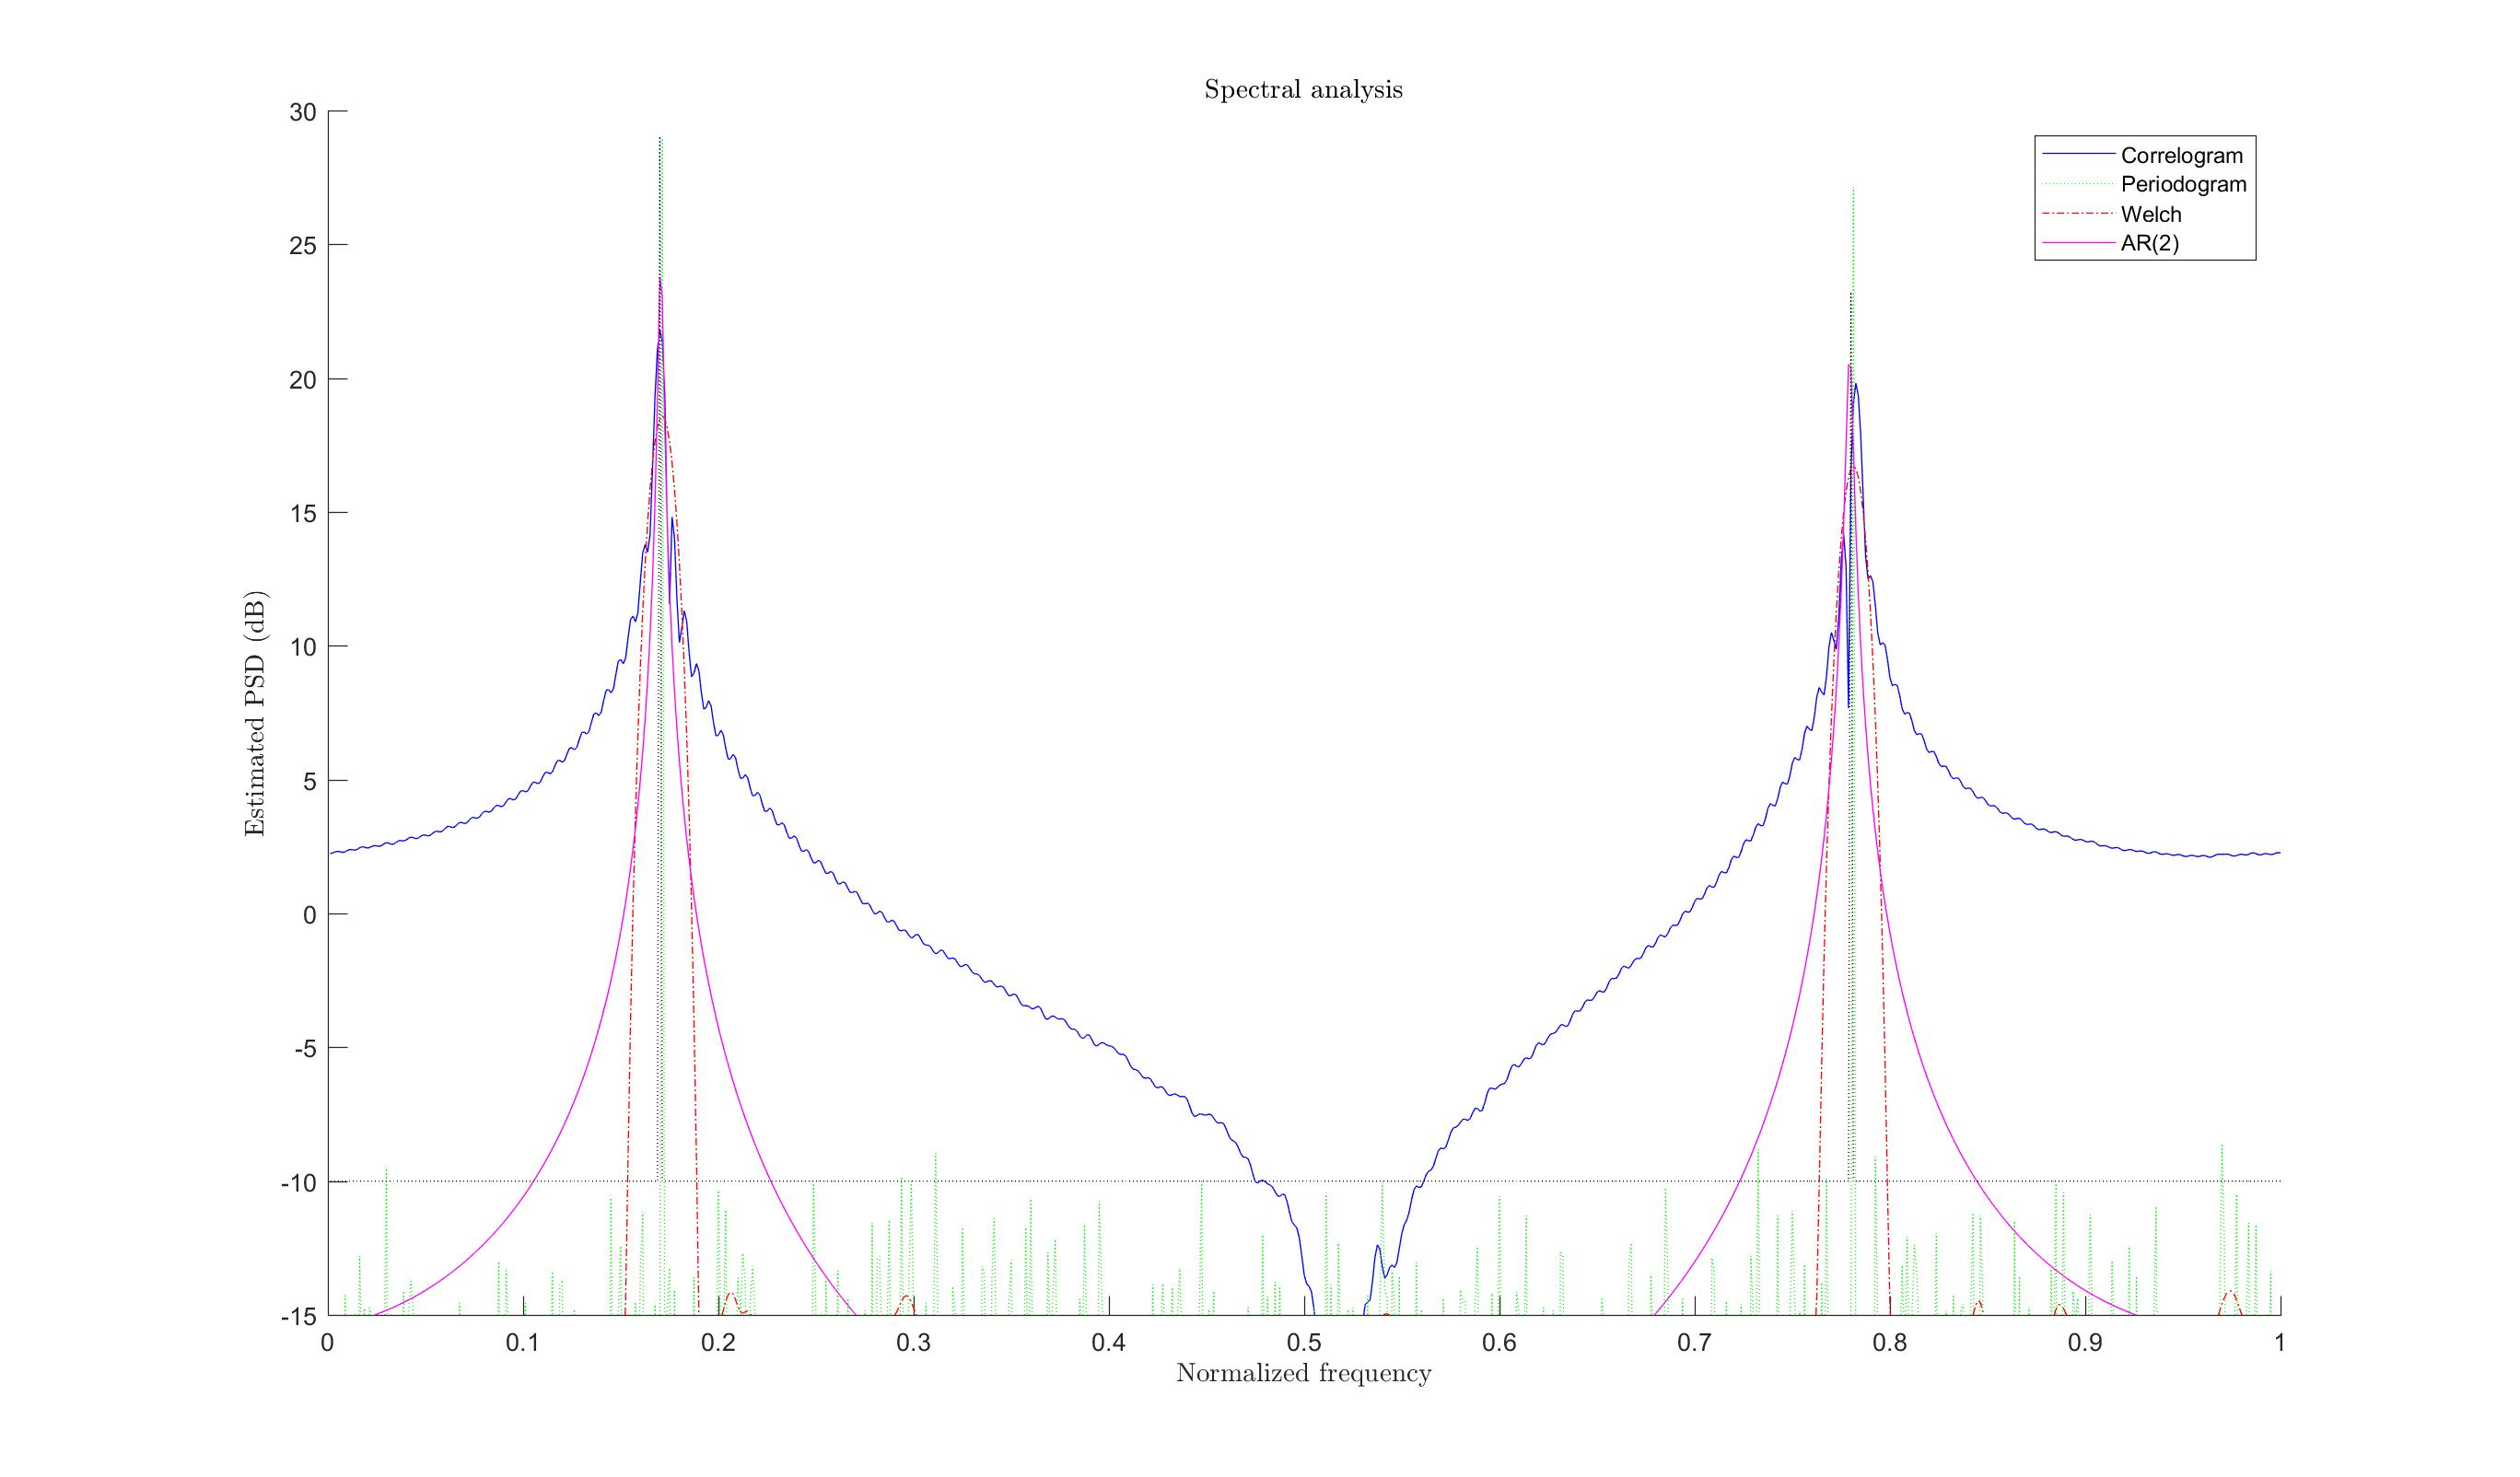
\includegraphics[width=14cm]{images/PSD_2.jpg}
	\caption{PSD estimates.}\label{PSD_2} 
\end{figure}

The parameters of the model are as follow. The order of the autocorrelation estimator for the Correlogram is $ N_{corr} = \lfloor K/5 \rfloor = 160 $, and the window used is a Bartlet window definde as
\begin{equation}\label{Bart}
w(k) = \begin{cases}
1-2 \left | \frac{k-\frac{D-1}{2}}{D-1} \right | \quad \quad k=0,1,...,D-1 \\
0 \quad \quad \quad \quad \quad \quad \quad \quad \quad\quad \quad \quad \quad \quad elsewhere
\end{cases}
\end{equation} 
This choise was taken by comparing the PSD estimates obtained with different windows, respectively: \textit{Hamming}, \textit{Rectangular} and \textit{Bartlett}. As shown in Figure [\ref{Welch_2}], the last one has a much more accurate behaviour.

\begin{figure}
	\centering
	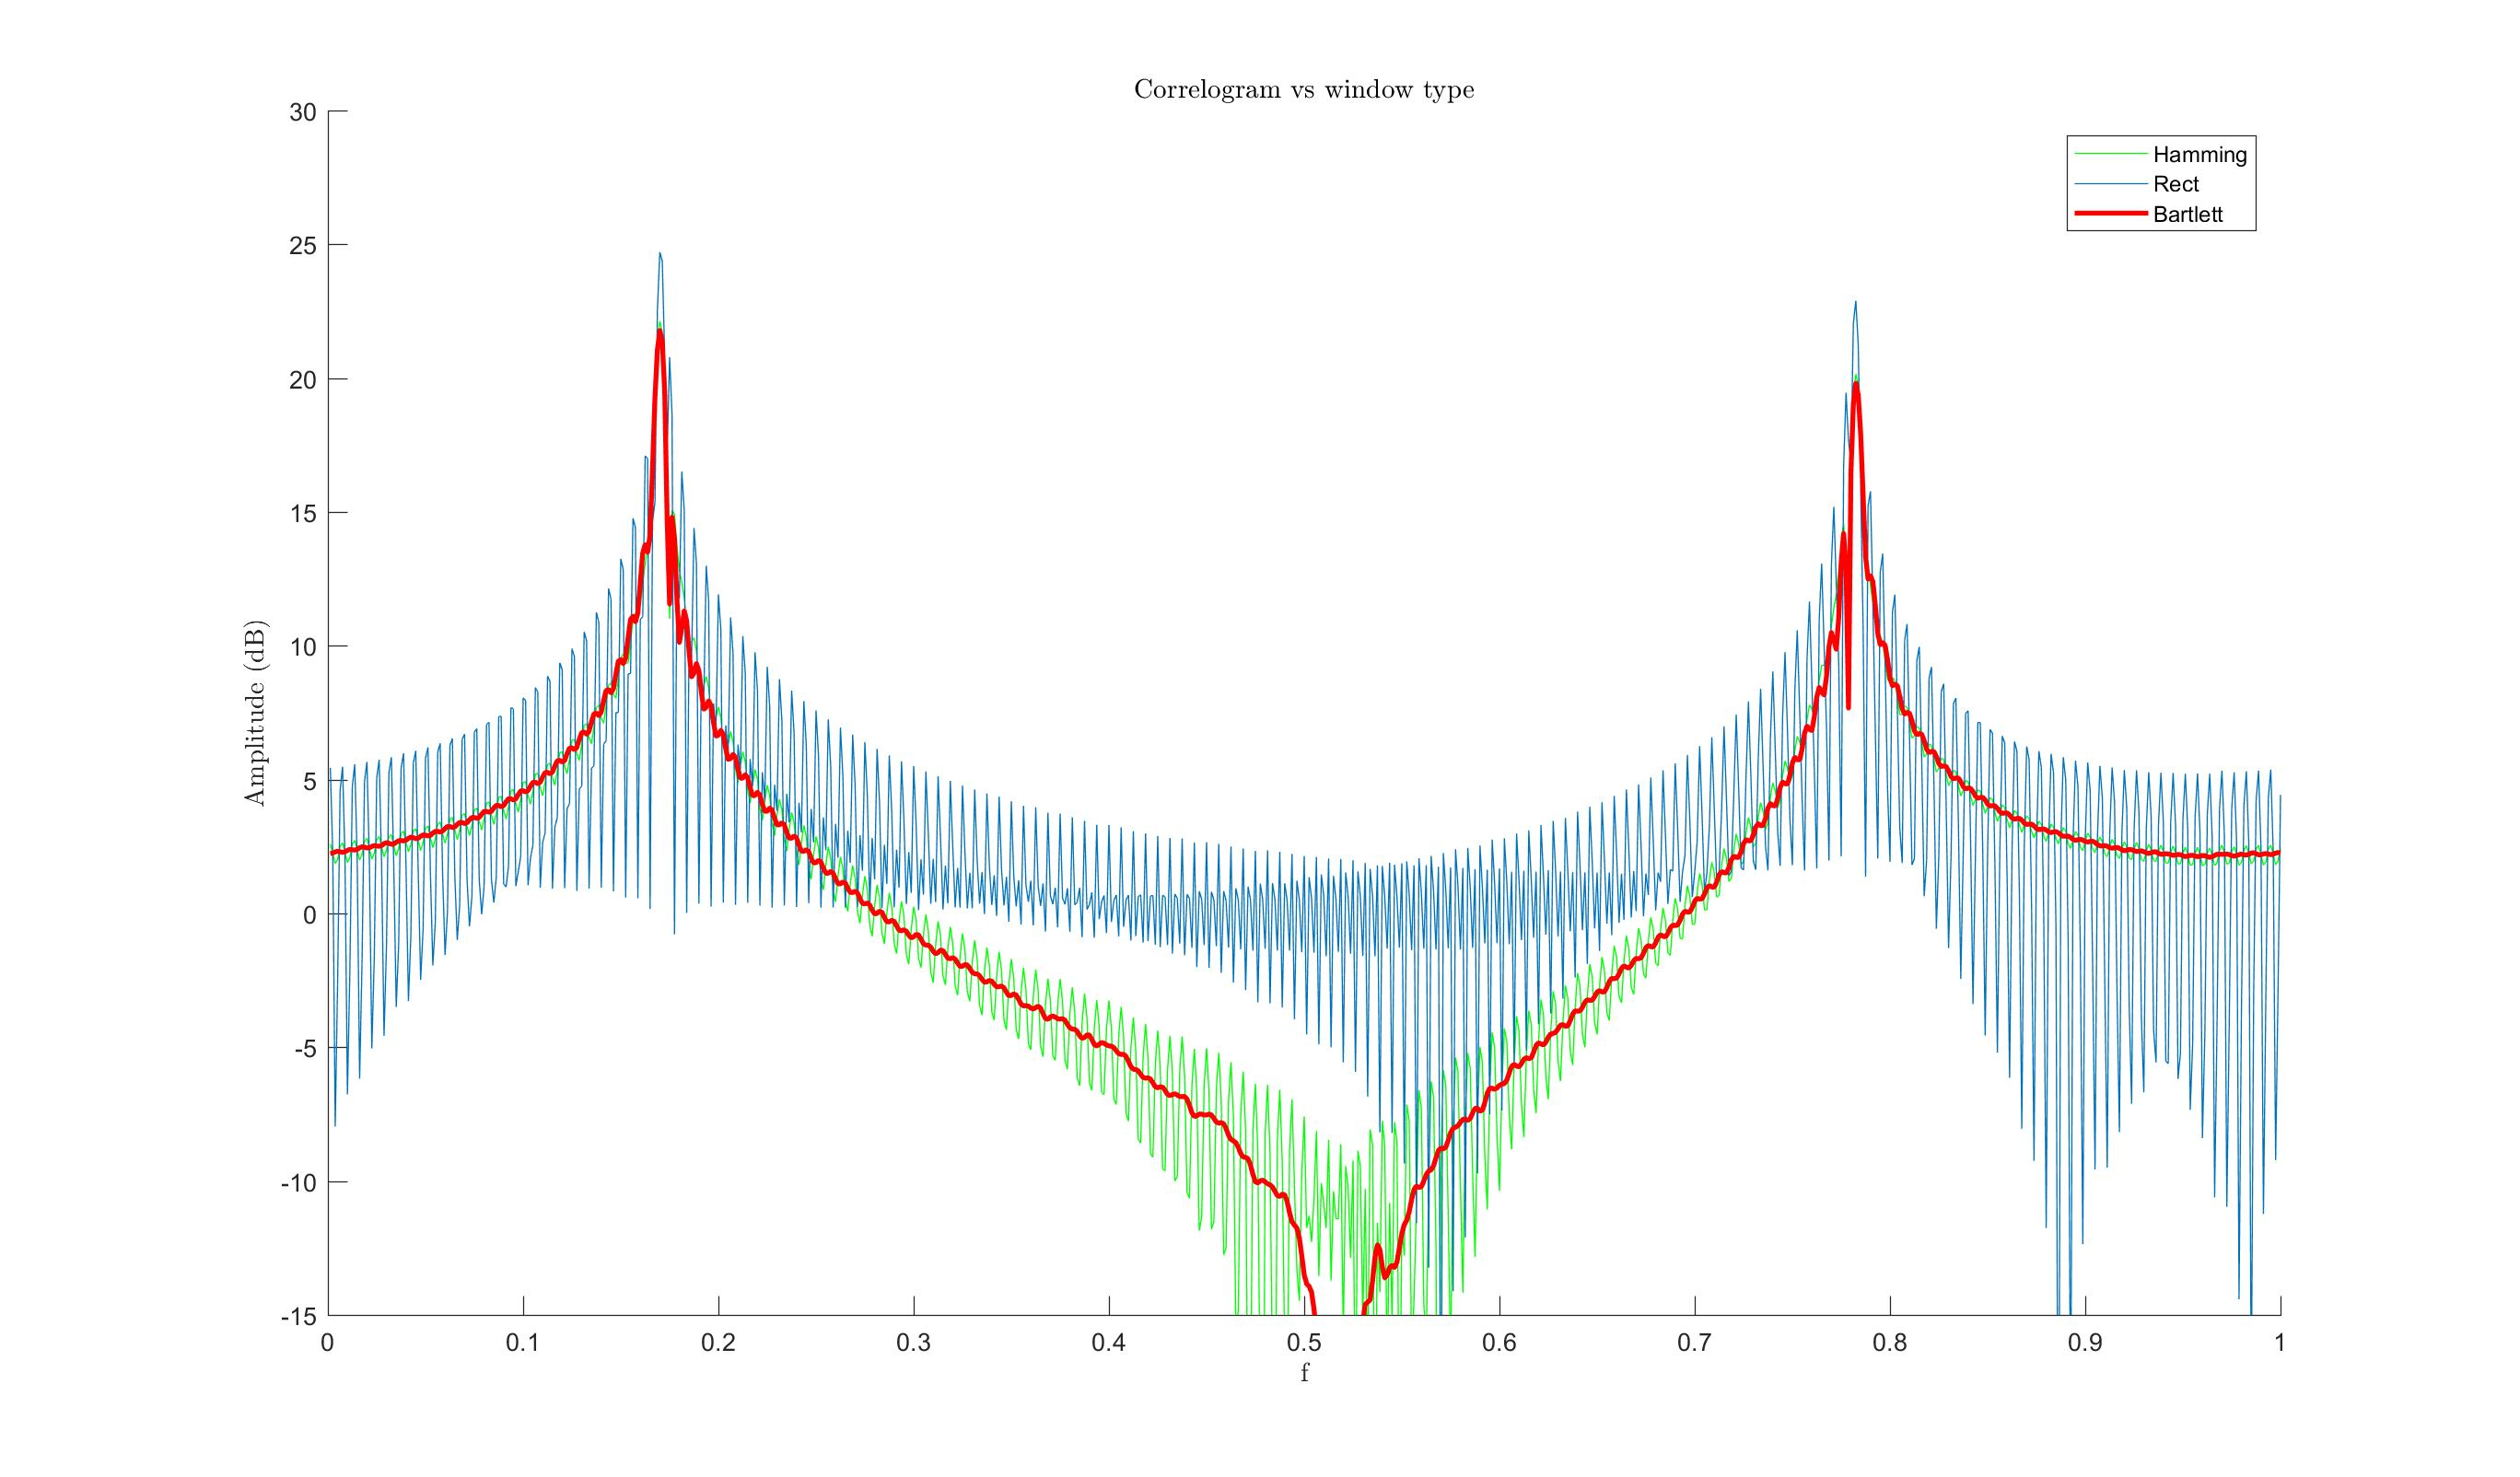
\includegraphics[width=14cm]{images/Corr_vs_window.jpg}
	\caption{PSD estimates.}\label{Welch_2} 
\end{figure}

For the Periodogram the window used is the rectangular one, while for the Welch Periodogram we set $D=??$ and $S=??$ using an Hamming window. Again, this choise was taken by comparing the PSD estimates with varying values of D and S, given in FIgure [\ref{WelchSD_2}]. Finally, the order evaluation for the AR model was carried out by analysing the behaviour of the noise variance $\sigma_w^2$ with varying N defined in eq. \ref{sigmaw} and graphically shown in Fig. [\ref{sigmavsN_2}]. Here it can be observed a knee in the function, which corresponds to a value of N=2.

\begin{figure}
	\centering
	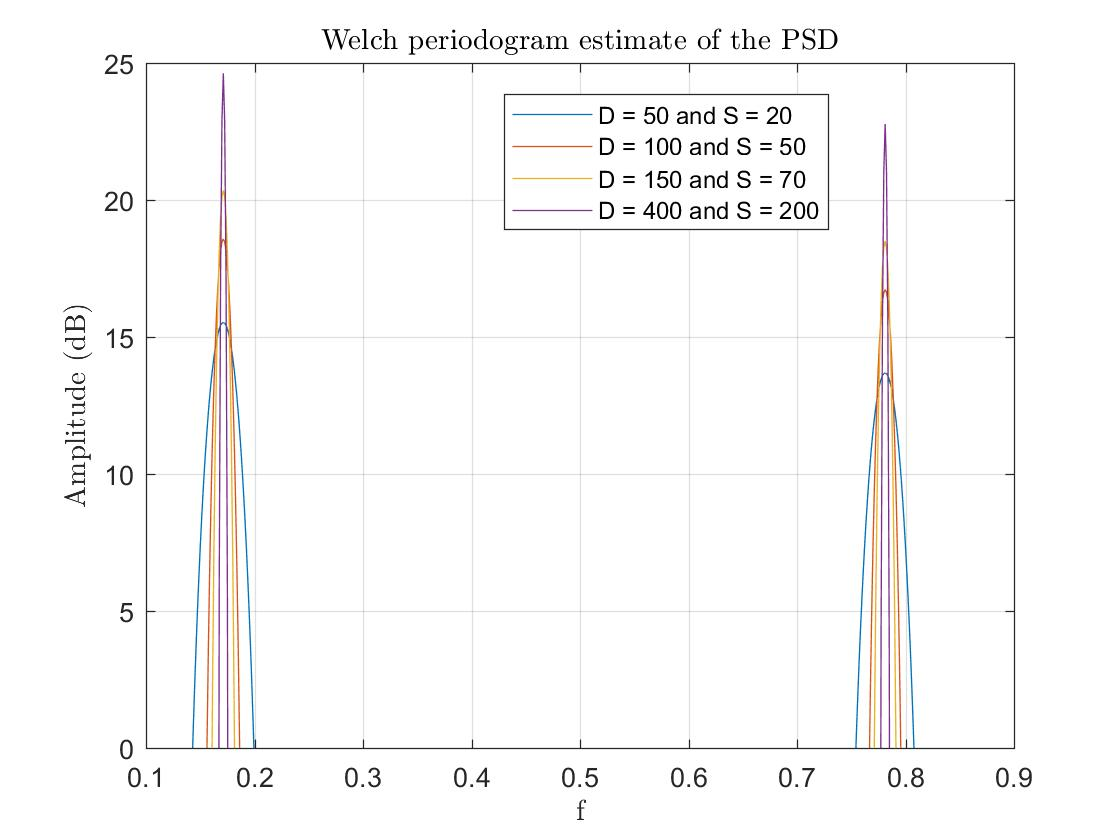
\includegraphics[width=14cm]{images/Welch_vs_SD_2.jpg}
	\caption{Welch periodogram estimates as a function of different values of D and S.}\label{WelchSD_2}
\end{figure}	
\begin{figure}[h]
	\centering
	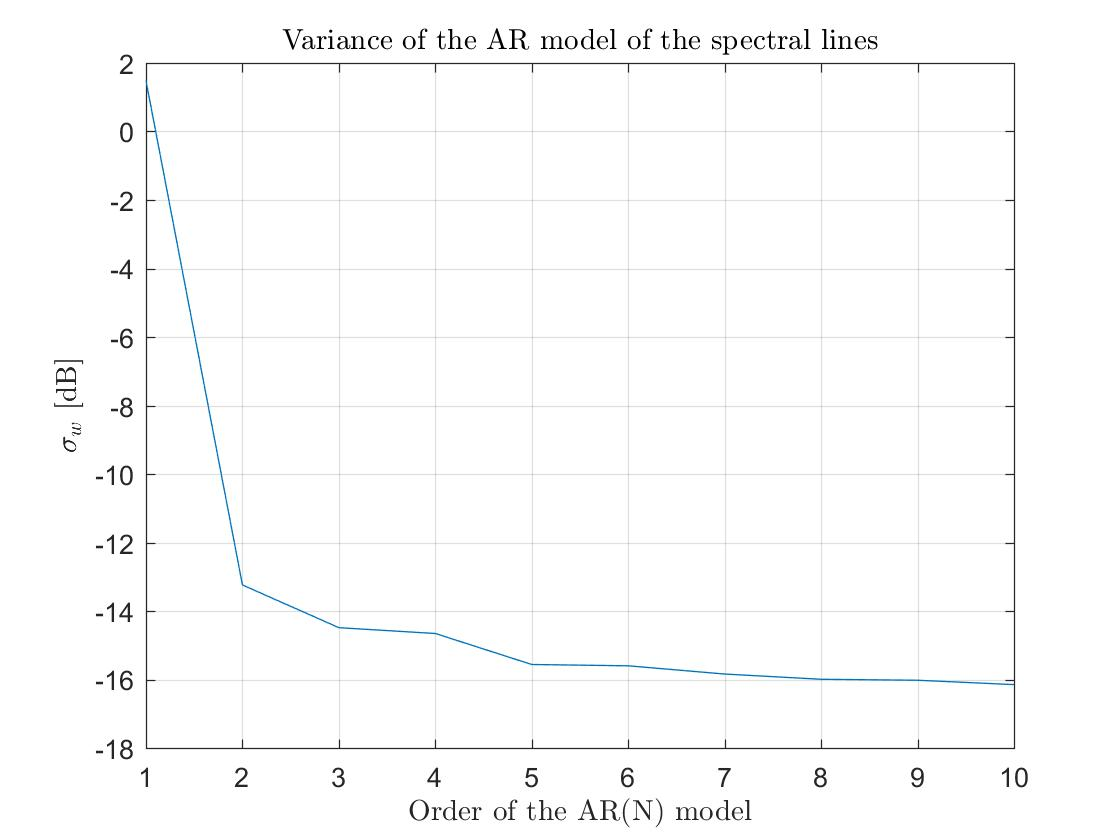
\includegraphics[width=14cm]{images/sigma_vs_N_2.jpg}
	\caption{Variance of the AR model white noise as a function of the order N.}\label{sigmavsN_2}
\end{figure}	


\clearpage
\section*{PROBLEM 3}
Given a discrete-time WSS random process \textit{x(k)} with zero mean at time \textit{k-1}, i.e. $\mathbf{x}^T(k-1) = [x(k-1), x(k-2), \dots, x(k-N)] $, the \textit{one-step forward predictor of order N} attempts to estimate the value of \textit{x(k)} using $\mathbf{x}^T(k-1)$. This problem can be solved by considering the signal $\mathbf{x}^T(k-1)$ as the input of a Wiener-Hopf filter of order N and $\textit{x(k)}$ as the reference signal. The solution is computed by the Wiener-Hopf equation 
\begin{equation*}
\mathbf{R}_N\mathbf{c}_{opt} = \mathbf{r}_N
\end{equation*}
It is important to underline that this solution holds if and only if the autocorrelation matrix $\mathbf{R}$ is invertible, i.e $\text{det}\mathbf{R}\ne0$. In this case the coefficent vector is optimum and it can be computed by
\begin{equation*}
\mathbf{c}_{opt} = \mathbf{R}^{-1}_N\mathbf{r}_N
\end{equation*}
Moreover, the minimum value of the cost function J is
\begin{equation*}
J_{min} = r_x(0)-\mathbf{r}_N^H\mathbf{c}_{opt}
\end{equation*}
Knowing that, given an AR process \textit{x} of order N, the optimum prediction coefficients $\mathbf{c}_{opt}$ coincide with the parameter $-\mathbf{a}$ of the process and, moreover, that $J_{min}=\sigma_w^2$, we can use the results of Problem 2 and get respectively:

\begin{itemize}
	\item N=2;
	\item $\mathbf{c}_{opt} = - \mathbf{a} = [+0,657 - 0,101i, -0,935 + 0,305i]$; 
	\item $J_{min}= \sigma_w^2 = r_x(0)+\mathbf{r}^H\mathbf{a}$.
\end{itemize}























\end{document}